% proposal.tex
\documentclass[main.tex]{subfiles}
\begin{document}
\chapter{Prediction of Mechanical Properties through Machine Learning} \label{ch:ml}

\section{Foreword} \label{sec:fw_ml}

The use of AM technologies to produce small batches of highly customized, complex parts in a reduced development cycle results extremely attractive to all industries. However, for AM parts to be fully adopted in industrial scenarios, engineers have to be able to confidently assess the structural integrity of the finished part under its intended loading conditions. This requirement is unfortunately not fully possible at the time this work was produced, partly because the mechanical properties of AM tend to be anisotropic, and partly because the relationships that exist between processing parameters, underlying physics of the process, and final mechanical part properties aren't fully comprehended. However, these obstacles present an interesting case for the application of Machine Learning (ML) techniques, where the inputs and outputs of a particular phenomenon are known, but there's a lack of explicit rules that indicate a relationship between the two. 

This work uses the Material Extrusion (ME) process as a case study for the application of ML techniques to predict the final mechanical properties of a printed part. Experimental work involved producing a variety of tensile coupons, developed under various printing conditions, and where the filament extrusion speed, filament extrusion force, and printing temperature were measured in real time using machines fitted with in-line sensors. These specimens were then tested up to tensile failure, and the collective data of printing parameters, measured process indicators, and mechanical tests results were used to train a Neural Network capable of predicting the tensile failure stress.

In the context of this dissertation, this represents an alternative method for part failure prediction to construction and evaluation of a failure envelope. However, it should be noted that both methods are not mutually exclusive, and as will be discussed, the author believes they can, and should, be combined. 

\section{Introduction} \label{sec:ml_intr}

The set of printing conditions that lead to an optimal part in terms of mechanical properties are not fully comprehended due to the nuances associated with the interacting effects of the processing conditions, material behavior, paired with a commonplace lack of standardization in the field of AM as a whole. However, recent advancements in processing power and algorithms have made it easier than ever to deploy Machine Learning (ML) solutions, and the intricacies of the processing-properties relationships of AM techniques represent an interesting case for development of a ML system. These excel in cases where the inputs and outcomes of a particular phenomena or task are known, but connecting the two through an explicit set of rules or relationships can result extremely complex and time consuming \cite{Chollet2018}. In this manner, ML models are \emph{trained}, as opposed to explicitly programmed, as illustrated in Figure \ref{fig:MLvsP_2}, where the differences between ML and traditional programming philosophies are compared. 

\begin{figure}[!htbp]
	\center
	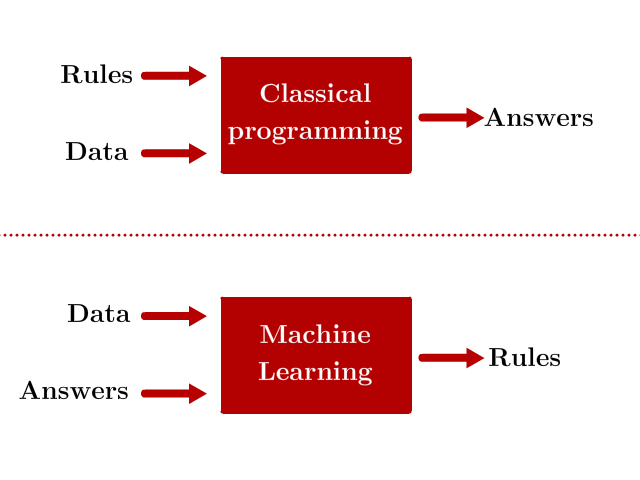
\includegraphics[height=6cm]{ML}
	\caption{Differences between traditional programming and machine learning. \cite{Chollet2018}} \label{fig:MLvsP_2}
\end{figure}

The potential to apply ML solutions in the field of AM has been noted by several authors \cite{Razvi2019,Meng2020}. Example cases include design-recommendation systems, topology optimization solutions, tolerancing and manufacturability assessment, and material classification and selection \cite{Razvi2019}. The specific algorithm applied for each case varied wildly depending on the nature of the task, but in general, Support Vector Machines (SVM) and Neural Networks (NN) appear to be the most prevalent solutions.

A Neural Network (NN) algorithm is effectively a facsimile of how biological neurons establish connections and communications with each other. In summary, the inputs of the problem are fed to a layer of nodes, or "neurons". Each node has itself a variety of connections to other neurons, and an associated weight and activation threshold, which if surpassed, triggers information transfer to its connections in subsequent layers. Finally, the information reaches the network stratus that estimates the outcome of whatever phenomena the model is trying to characterize, traditionally named the output layer \cite {Chollet2018, IBMCloudEducation2020, Geron2019}. The weights and activation thresholds of each node are iteratively tuned as the NN architecture is exposed to a training data set, while also being compared to a separate set of data points used for validation. Once the accuracy of the model reaches its desired value, the underlying communication between the neurons is capable of making predictions based on what the input layer is perceiving. A schematic of a NN can be seen in Figure \ref{fig:NN}. The particular NN shown in this image is called a Deep Neural Network, as the number of layers of nodes surpasses three \cite{IBMCloudEducation2020}. This type of architecture tends to be reserved for computationally complex tasks, such as text recognition or image processing.  

\begin{figure}[!htbp]
	\center
	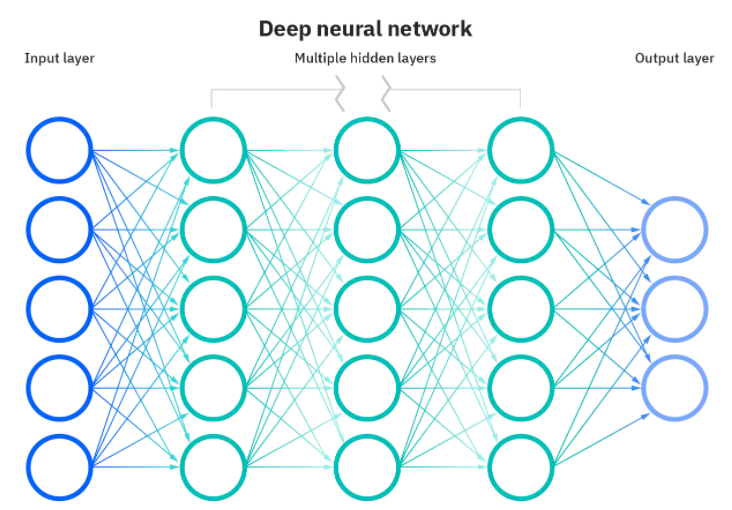
\includegraphics[width=0.8\linewidth, keepaspectratio]{NN_scheme}
	\caption{Schematic of a NN \cite{IBMCloudEducation2020}} \label{fig:NN}
\end{figure}

The capability of NNs to model complex behaviors is rooted in the mathematical operations that happen behind the scenes. Each neuron behaves effectively as its own mini linear regression model, represented in Equation \ref{eq:neuron}. Here $X_{i}$ and $W_{i}$ represent one of the node's $m$ inputs and its associated weight respectively.  

\begin{equation} \label{eq:neuron}
	\sum_{i=1}^{m} W_{i}X_{i} + bias = z
\end{equation}  

The weighed sum of the inputs can then be used as is, or passed through an activation function. This signals the generation of an output that can then be used at face value, or transmitted to subsequent nodes if a threshold is surpassed. Assuming for the purposes of this example that the threshold is zero, and the activation function is the Heaviside step function, the output of a neuron can be computed as:

\begin{equation} \label{eq:heav}
	Heaviside(z) = \begin{cases}
		1 & \text{if } z \geq 1\\
		0 & \text{otherwise}
	\end{cases}
\end{equation}


Concatenating nodes in a forward fashion creates the concept of levels, or \emph{layers} in a network. When all neurons in a layer are fully connected to the nodes in the previous level, this is typically named a \emph{Dense} layer. Arranging more than one dense layer in series results in a NN \cite{Chollet2018, Geron2019}. 

The weights of each neuron are iteratively tuned in a process that involves penalizing the model using a loss function, that compares the predictions of the model with true output values using example data. This process is effectively an optimization task where the goal is to minimize the loss function. A schematic of the process can be seen in Figure \ref{fig:NN_it}, using a two layer network architecture as an example.

\begin{figure}[!htbp]
	\center
	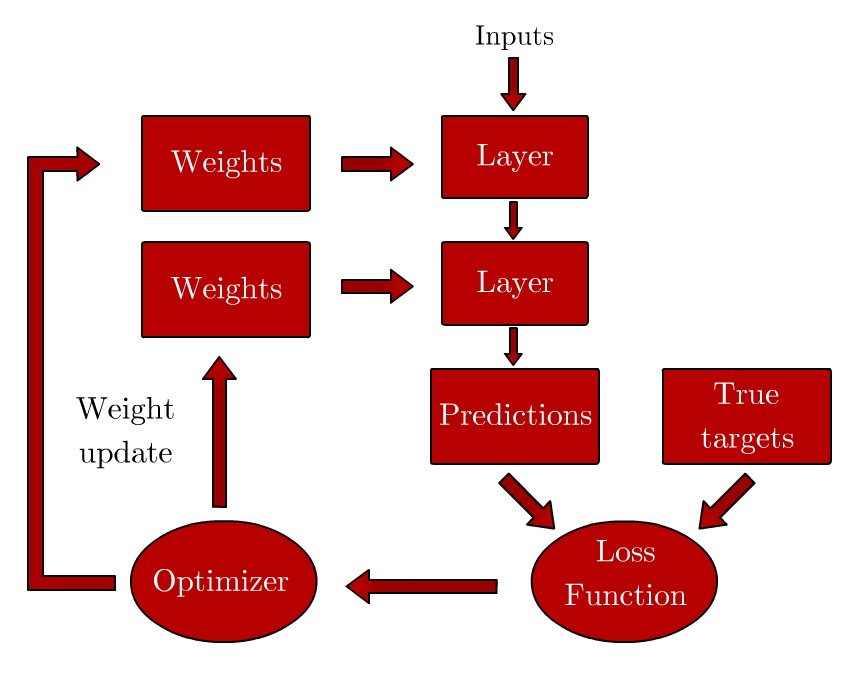
\includegraphics[width=0.7\linewidth, keepaspectratio]{weight_ML}
	\caption{Iterative process of NN parameter tuning \cite{Chollet2018}} \label{fig:NN_it}
\end{figure}

Unfortunately, while NNs are powerful, highly adaptable predictive models, the contributions of each input are usually hidden behind a veil of complexity that makes it almost impossible for the user to comprehend what is happening behind the scenes \textemdash fittingly, much in the same way we do not fully understand how brains and cognition work. Luckily, recent developments in interpretability of models allow a peek inside the inner machinations of a NN, normally considered a "black box" model. Of particular interest, is the application of Shapley values to aid in the understanding of how a trained ML model is affected by each of its inputs.

A Shapley value is a concept that stems from game theory. To paraphrase and over-simplify the formal definition, if a coalition $C$ collaborates to produce a value $V$, the Shapley value is simply how much each member of the coalition contributed to its final output \cite{Shapley+2016+307+318, Molnar2021}. For instance, it can determine the average contribution of each player, to the output of the team in a game; how much profit did each members of a corporation produce throughout a year; and more importantly for the contents of this work, \emph{how much is each input of a model contributing to its output}. The formal mathematical definition is computationally expensive and escapes the scope of this work, but a numerical approximation using Monte-Carlo sampling, proposed by \v{S}trumbelj et al. \cite{Strumbelj2014} states that, for any model $f$ capable of making a prediction using the vector $x$ with $M$ features as an input, the Shapely value ${\phi}_{j}$ for that particular input can be approximated as follows:

\begin{equation} \label{eq:shap_MC}
	\frac{1}{M}\sum_{m=1}^{M} (\hat{f}(x^{m}_{+j})-\hat{f}(x^{m}_{-j})) = \hat{\phi}_{j}
\end{equation}

Where $\hat{f}(x^{m}_{+j})$ and $\hat{f}(x^{m}_{-j})$ represent predictions made by the model using two synthetic datapoints, constructed using a random entry from the database, called $z$. The former term is the instance of interest, but all values in the order after feature $j$ are replaced by feature values from the sample $z$. Similarly, the latter term, $\hat{f}(x^{m}_{-j})$ is constructed in the same manner as $\hat{f}(x^{m}_{+j})$, but it also replaces feature $j$ by its counterpart from datapoint $z$ \cite{Molnar2021}. 

To facilitate its applicability to ML, Lundberg and Lee created the SHAP (Shapley Additive Explanations) method to explain individual predictions. The SHAP method effectively models "any explanation of a model's prediction as a model itself", termed an \emph{explanation model} \cite{NIPS2017_8a20a862}. Thus, any model $f$ can be approximated using an explanation model $g$ using the equation below, where $z'$ represents a simplified version version of input $z$, such that $z = h_{x}(z')$:

\begin{equation}
	g(z')\approx f(h_{x}(z'))
\end{equation}

Finally, for the purposes of SHAP, the explanation model of choice has each effect $\phi_{i}$ attributed to a feature, and the sum of the effects of all feature attributions approximates the outputs of the original model $f$. This explanation model is represented by the equation below.

\begin{equation} \label{eq:SHAP}
	g(z') = \phi_{0} + \sum_{m=1}^{M} \phi_{i}z_{i}^{'}
\end{equation}

Using Equations \ref{eq:shap_MC} and \ref{eq:SHAP}, one can use Shapley values to identify the importance of features in a respective model. This allows the user to make decision pertaining to the architecture of the model, as well as appreciating the impact a particular input can have on the output of the model \textemdash something that would be difficult to do without this resource. These mathematical principles are built into the SHAP Python library out of the box \cite{NIPS2017_8a20a862}.

Given the factors outlined this far, the fundamental goal of this research is to predict ME part mechanical performance by training a NN with data generated through the use of sensors built into a 3D printer. This tool can then be used to predict final mechanical properties of the part based on the data generated during the print. The features selected as controlled variables for the Design of Experiments (DoE) were Layer Height (LH), Nozzle Diameter (ND), and Print Speed (PS). These parameters were chosen based on previous research that shows that these slicing parameters had a tangible impact upon the final tensile strength of ME coupons \cite{Koch2017, Rankouhi2016}. Coupons are to be printed in both $0\deg$ and $90\deg$ orientations so the model can predict both the highest and lowest possible mechanical properties of each particular printing condition. Additional attention will be paid to the changes in required print force as these parameters are varied to produce the mechanical test coupons. The models produced through this research will be analyzed using Shapley values through the SHAP method to draw conclusions regarding the impact of the selected features of the model.

\section{Experimental Methods} \label{sec:ml_meth}

\subsection{Design of Experiments}\label{ssec:doe}

The target values of the predictive NN are the required average extrusion force ($F$) for the print, Tensile Strength of the coupon ($\sigma_{t}$), and the Elastic Modulus of the sample ($E$). In order to capture a variety of printing conditions, the selected controlled variables were varied in a three level, full-factorial experimental layout, which can be seen in Table \ref{tab:ml_doe}. Each printing condition was replicated 2 times to account for variability in the samples, and all combinations were reproduced using both a $0^{\circ}$ and $90^{\circ}$ orientation.

\begin{table}[!htbp] %Fixates table so that it doesn't randomly jump around between pages
	\renewcommand{\arraystretch}{1.5}
	\centering
	\caption{Controlled variables in the Design of Experiments}
	\begin{tabular}{ c c } 
		\toprule
		\textbf{Variable} & \textbf{Levels} \\
		\midrule
		 Layer Height (LH) [$mm$]  &  0.1, 0.2, 0.4\\
		 Nozzle Diameter ($D_{N}$) [$mm$] & 0.3, 0.4, 0.8\\
		 Print Speed (PS) [$mm/min$] & 1200, 2400, 3600\\
		\bottomrule
	\end{tabular}
	\label{tab:ml_doe}
\end{table}

\subsection{Equipment and methods}\label{ssec:datag}

A set of 4 identical customized ME 3D printers (Minilab by FusedForm, Colombia) fitted with sensors capable of recording the force exerted by the filament upon the nozzle, discrete measurements of temperature, and changes in the extruded length over time were used to reproduce a variety of tensile coupons. A schematic of the printer setup can be seen in Figure \ref{fig:print_setup}. The data was collected using an Arduino board sampling at a frequency of 5 Hz, connected to MATLAB for visualization, processing, and logging. A Buttersworth filter was applied to amplify the signal-to-noise ratio of the outputs of the system. The force sensor and encoder have an innate uncertainty of $\pm20 g$, and $200$ Pulses per Revolution respectively. The code for the data acquisition and filtering can be found in Appendix \ref{ch:daq}. A random set of printing conditions were reproduced on all printers to monitor printer-to-printer variability.

\begin{figure}[!htbp]
	\center
	\includegraphics[height=7cm]{forcesetup}
	\caption{Schematic of modified ME printer with sensors} \label{fig:print_setup}
\end{figure} 

To minimize the impact of lurking variables, the filament was extruded in-house, using the SABIC Cycolac MG94 ABS material, using an extrusion line that maintained the filament diameter within the target of $1.75 \pm 0.05 \text{ mm}$ using a vacuum assisted water bath, a laser micrometer, and a conveyor belt in a control loop. Each filament was dried for a minimum of 3 hours at $65^{\circ}C$ and kept in a drybox attached to the printer during manufacturing. Bed leveling was performed after 10 prints, or each time a change in material or nozzle was necessary. Nozzles were burned off in a furnace every time they were switched to minimize the influence of clogging.

Each print consisted of four rectangular tensile coupons of dimensions $25 \text{ mm}$ by $100 \text{ mm}$ by $3.2 \text{ mm}$, chosen to strike a balance between being relatively quick to print, having at least $50\text{ mm}$ of gauge length, and fitting in the jaws of the tensile testing equipment. Each coupon was printed in a part-by-part manner (as opposed to having a single layer of the print construct a slice of all coupons), to approximate real printing behavior as much as possible. Since a single experimental run yielded four coupons, post-processing was required to separate the force-data-speed pairings for each specimen. A pause was introduced between each part that would allow discerning when one specimen print was finished, and the next started. A schematic of the process is shown in Figure \ref{fig:print_dia}. 


\begin{figure}[!htbp]
	\center
	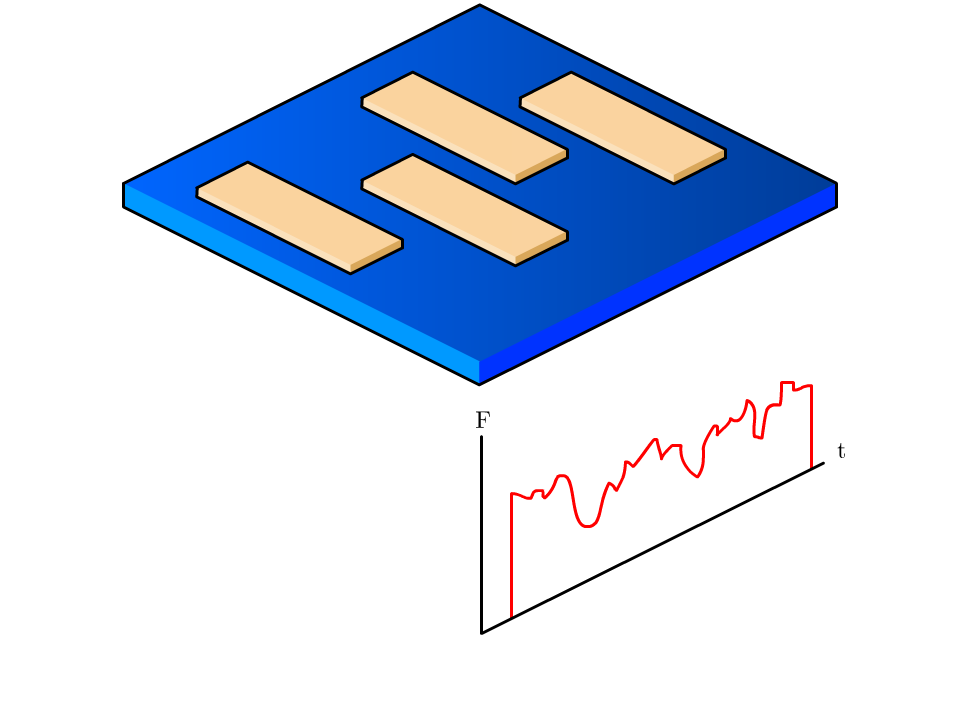
\includegraphics[height=6cm]{coupon_print_diagram}
	\caption{Schematic of print experiment} \label{fig:print_dia}
\end{figure}

Additionally as an exploratory experiment, the geometric information of the filament was collected and paired to the rest of the information stemming from the in-line measurements of a handful of prints, to assess if variations in the filament geometry resulted in notable changes in the required print force. This data was attained through the use of a laser micrometer and a conveyor belt, pulling the material at a constant, known speed. The process yielded discrete measurements of the filament diameter and ovality as a function of filament length and time. A schematic of the process can be seen in Figure \ref{fig:FD}.  

\begin{figure}[!htbp]
	\center
	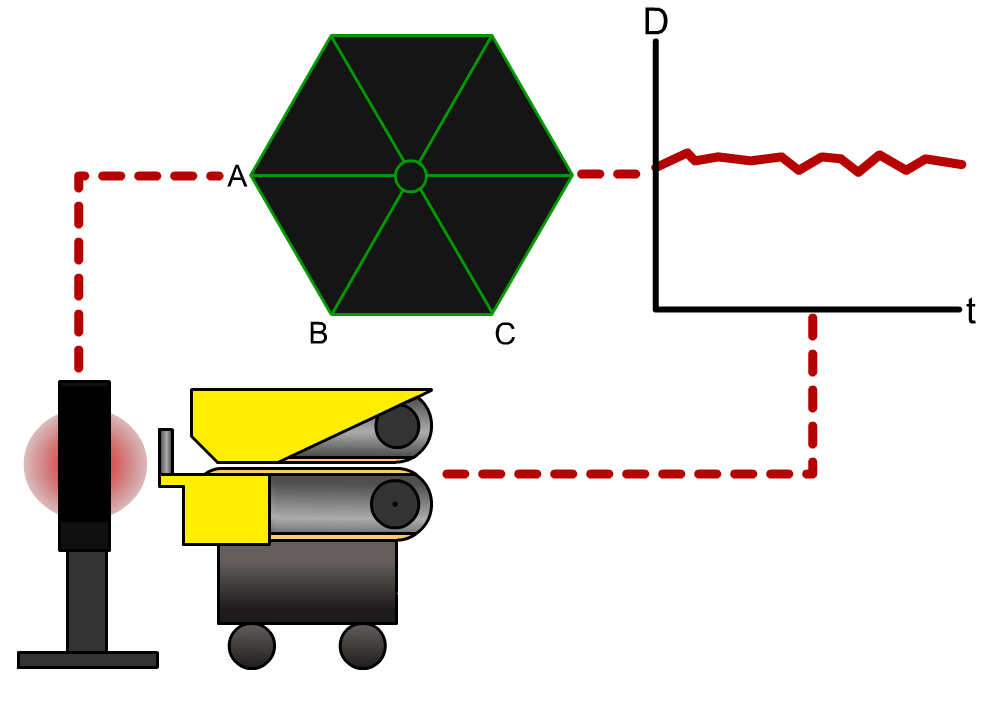
\includegraphics[width=0.6\linewidth]{filament_measurement}
	\caption{Filament geometry information, acquired through a laser micrometer } \label{fig:FD}
\end{figure}

Tensile testing was performed using an Instron 5967 dual column universal testing machine, fitted with a 30 kN load cell. All data acquisition was handled through the accompanying Instron Bluehill 3 software. A movement speed of 5 mm/min was used to deform the 50 mm gage section of the specimens, with all deformations being logged using an extensometer. To protect the samples from excessive gripping force, emery cloth tabs were used \cite{Capote2017}. This setup can be seen in Figure \ref{fig:testsetup}. The final step of the process involved matching the printing data to its corresponding mechanical test results, and assembling everything in a single database. This was done using a Python code that would search the directory of the raw data and construct a \emph{.csv} file including all the pertaining information of an experimental run in a row. This step is necessary for the ML code to quickly read and understand the information that it is attempting to model. This code can be found in Appendix \ref{ch:csv}. 

\begin{figure}[h]
	\center
	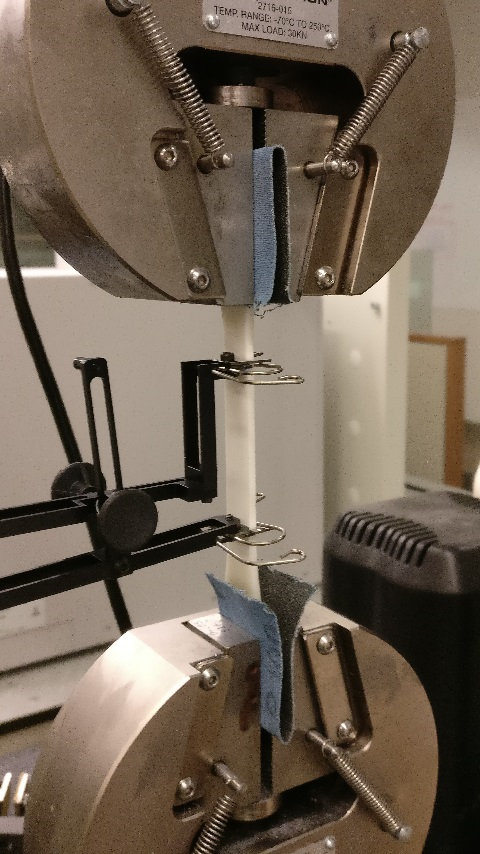
\includegraphics[height=8cm, keepaspectratio]{tensgrip}
	\caption{Tensile testing setup} \label{fig:testsetup}
\end{figure} 

An additional metric that can aid in identifying underlying systematic issues or relationships between the print and its mechanical properties is comparing the expected filament speed against its experimentally measured counterpart. The theoretical filament speed can be calculated using a simple volumetric balance. The volume of an extruded bead can be approximated as $ND. D_{N}. l$, where $l$ represents the bead length. Given that mass must be conserved, this implies that the volume of the bead $V_{out}$ must be equal to the volume supplied by the incoming filament $V_{in}$ resulting in the equation below, where $D_{f}$ and $L$ represent the filament diameter and length supplied to extrude the bead respectively:

\begin{equation} \label{eq:v_b_1}
	V_{out}= LH . D_{N} . l = V_{in} = \frac{\pi . D_{f}^2 . L}{4}
\end{equation}

Manipulating Equation \ref{eq:v_b_1} to solve for $L$ results in:

\begin{equation} \label{eq:v_b_2}
	L = \frac{LH. D_{N}. l. 4}{\pi . D_{f}^2}
\end{equation}

Now, one can use the expected time to print a bead of dimensions $l$ to solve for the expected filament speed $S_{t}$.

\begin{equation} \label{eq:v_b_3}
	t = \frac{l. 60 s}{PS}
\end{equation}

Finally, combining Equations \ref{eq:v_b_2} and \ref{eq:v_b_3} yields the theoretical filament speed, $S_{t}$. The equation includes a conversion factor to solve in units of $mm/s$.

\begin{equation} \label{eq:v_b_4}
	S_{t}=\frac{4. LH. D_{N}. PS}{\pi . D^2 . 60s}
\end{equation}

\subsection{Experimental Results}\label{ssec:ml_exp_r}

\subsubsection{Effect of Variations in Filament Diameter upon Extrusion Measurements}

The effect of fluctuations in the filament geometry upon the required extrusion force is unknown, but are expected to be proportional given the current filament extrusion models. As an exploratory experiment, the data stemming from the measurements of the laser micrometer were matched to its corresponding data readings resulting from the printer sensors. The condition chosen to test this experiment was $LH = 0.2 \text{ mm}$, $D_{N} = 0.4 \text{ mm}$, $PS = 2400 \text{ mm/min}$. Matching the filament diameter and ovality measurements to the corresponding speed and force readings from the sensors resulted in inconclusive results. This can be seen in Figure \ref{fig:f_O_D}, where the force remains nearly constant despite the variations of filament diameter and ovality. 

\begin{figure}[!htbp]
	\center
	\subfloat[Effect of ovality on measured filament force \label{fig:O_f}]{%
		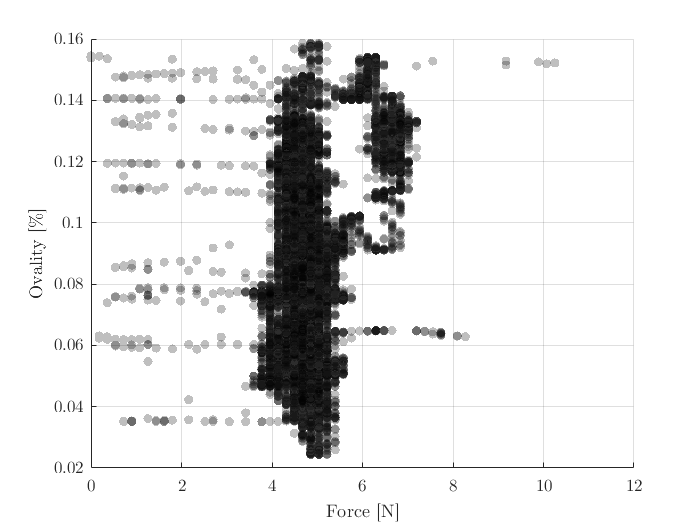
\includegraphics[width=0.8\linewidth, keepaspectratio]{force-ovality}
	}
	\linebreak
	\subfloat[Effect of diameter on measured filament force \label{fig:D_f}]{%
		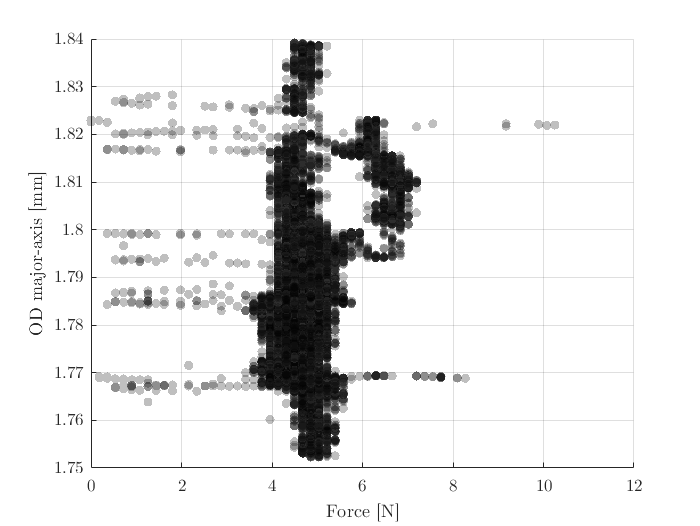
\includegraphics[width=0.8\linewidth, keepaspectratio]{force-OD}
	}
	\caption{Effect of filament geometry on extrusion force} \label{fig:f_O_D}
\end{figure}

Pairing the geometric information of the filament to its corresponding print data proved to be an extremely time consuming task, given that both sets of information came from different devices, and that in order to get proper matching, the starting point of the print had to be accurately pinpointed as length zero. The inconclusive nature of  these results, and the additional time required to further explore this phenomena lends itself well to be explored as future work, with a device that measures the filament geometry directly within the printer, as to facilitate exploring trends over more printing conditions. 

\subsubsection{Printer Sensor Data Analysis}

Generally speaking, the average measured filament speed was very consistent within a particular print condition. Standard deviation for filament print speed data varies between $6.6x10^{-4}$ and $1.8 \text{mm/s}$. In contrast, the measured print force varied drastically between experimental runs, and even within the same print. As an example, four print coupons produced in a single print using $LH= 0.2 mm, D_{N} = 0.4 mm, PS = 2400 mm/min$ had average forces of $792.66, 611.52, 516.86, \text{and } 554.91$ g respectively. The standard deviation of the measured print force ranged between $16$ and $475\text{ g}$, with higher variability observed in prints involving the smallest nozzle diameter combined with the largest layer height. The conditions selected to test experimental reproducibility between printers showed no higher variability than fluctuations of measured force and filament speed within the same printer, with the highest discrepancy between printers in the range of $100 \text{ g}$ and $1x10^{-3} \text{ mm/s}$ respectively. 

For most conditions, the measured filament speed approximated the theoretical value fairly closely, with most specimens achieving a real-to-expected speed ratio between $0.95-0.97$. However, a couple of generalizations can be made for certain combinations of experimental values that had ratios below $0.9$. These involved the fastest $PSs$ combined with a $LH$ that was larger than the $D_{N}$, namely, a $0.3 \text{ mm} N_{D}$ paired with either a $0.4 \text{ mm}$ or $0.8 \text{ mm}$ $LH$. It is believed that this is caused by having filament force requirements that go beyond the capabilities of the machine, resulting in slippage at the drive wheel of the system. This effect was present in more conditions in the $90^{\circ}$ orientation, in particular, conditions that involved the $3000 mm/min$ gantry speed. This is theorized to be caused by a shorter travel distance between contiguous beads, implying that the acceleration of the system was not sufficient to attain the desired filament speed before the toolpass required a change in direction. 

\subsubsection{Tensile Testing Results}

Box-whisker plots were used to identify outliers in the data using the Interquartile Range method (IQR). Once an outlier was detected, the entry of the database was replaced with the average of that particular condition. This was done as a way to avoid data-loss without introducing noise or bias to the expected response. An example plot can be seen in Figure. %TODO
%INSERT BOX AND WHISKERS PLOT HERE

\subsection{Statistical Analysis}\label{ssec:fact}
Analysis of the data was performed in two ways. First using the entire data set to develop a Pearson correlation matrix, and secondly, analyzed as a full-factorial experimental design, separating the data set in  two: one for each printing orientation. 

The Pearson correlation matrix allows discerning whether variables and a response may posses a linear correlation with each other, with a coefficient of 1 (or -1) indicating perfect linear correlation. It should be noted that a low Pearson index does not mean no correlation, it simply implies that the relationship may not be linear in nature \cite{Geron2019}. The resulting matrix can be seen in \ref{tab:pearson}. Here it can be seen that out of all responses of interest, only the force shows high likelihood of linear correlation with the $LH$, $D_{N}$, $PS$, and $S$.

\begin{table}[!htbp]
	\renewcommand{\arraystretch}{1.5}
	\centering
	\caption{Pearson Correlation Matrix}
	\begin{tabular}{l|llllllll}
		\toprule
		& O      & LH     & $D_N$  & PS     & S      & F      & E      & $\sigma_{T}$ \\
		\midrule
		O            & 1      & -0.056 & 0.063  & 0.042  & 0.003  & 0.044  & -0.108 & -0.835       \\
		LH           & -0.056 & 1      & -0.018 & -0.011 & 0.6    & 0.583  & -0.097 & -0.077       \\
		$D_N$        & 0.063  & -0.018 & 1      & 0.051  & 0.522  & -0.367 & -0.232 & -0.267       \\
		PS           & 0.042  & -0.011 & 0.051  & 1      & 0.464  & 0.403  & -0.081 & -0.1         \\
		S            & 0.003  & 0.6    & 0.522  & 0.464  & 1      & 0.398  & -0.209 & -0.176       \\
		F            & 0.044  & 0.583  & -0.367 & 0.403  & 0.398  & 1      & 0.015  & -0.014       \\
		E            & -0.108 & -0.097 & -0.232 & -0.081 & -0.209 & 0.015  & 1      & 0.215        \\
		$\sigma_{T}$ & -0.835 & -0.077 & -0.267 & -0.1   & -0.176 & -0.014 & 0.215  & 1\\
		\bottomrule          
	\end{tabular}
\end{table} \label{tab:pearson}

The factorial experimental analysis of variance (ANOVA) yields results relating to how the input variables can have direct or interacting effects upon the measured response. Starting with the $0^{\circ}$ orientation, the ANOVA test determined that using a $95\%$ confidence interval, the print force is directly affected by the main effects of the selected control variables, as well as its two and three way interaction effects. A similar conclusion can be drawn for the tensile strength. Interestingly, only the Nozzle Diameter and the Print Speed have tangible main and interaction effects upon the Elastic Modulus. Results can be seen in Table \ref{tab:anova_0}, where $*$ denotes a p-value lower than $0.001$.

\begin{table}[!htbp]
	\renewcommand{\arraystretch}{1.5}
	\centering
	\caption{Summary ANOVA table of $0^{\circ}$ experiments}
	\label{tab:anova_0}
	\begin{tabular}{ccccccc}
	\hline
	& \multicolumn{2}{c}{F}                 & \multicolumn{2}{c}{E}                & \multicolumn{2}{c}{$\sigma_{T}$} \\ \hline
	\multicolumn{1}{c|}{Effect}        & f      & \multicolumn{1}{c|}{p-value} & f     & \multicolumn{1}{c|}{p-value} & f              & p-value         \\
	\multicolumn{1}{c|}{LH}            & 349.41 & \multicolumn{1}{c|}{*}       & 2.17  & \multicolumn{1}{c|}{0.117}   & 382.56         & *               \\
	\multicolumn{1}{c|}{$D_{N}$}       & 361.45 & \multicolumn{1}{c|}{*}       & 11.30 & \multicolumn{1}{c|}{*}       & 3.44           & 0.034           \\
	\multicolumn{1}{c|}{PS}            & 213.43 & \multicolumn{1}{c|}{*}       & 9.37  & \multicolumn{1}{c|}{*}       & 9.17           & *               \\
	\multicolumn{1}{c|}{$LH*D_{N}$}    & 15.05  & \multicolumn{1}{c|}{*}       & 1.17  & \multicolumn{1}{c|}{0.326}   & 16.10          & *               \\
	\multicolumn{1}{c|}{$LH*PS$}       & 44.50  & \multicolumn{1}{c|}{*}       & 3.21  & \multicolumn{1}{c|}{0.014}   & 30.16          & *               \\
	\multicolumn{1}{c|}{$D_{N}*PS$}    & 4.77   & \multicolumn{1}{c|}{0.001}   & 1.22  & \multicolumn{1}{c|}{0.304}   & 35.95          & *               \\
	\multicolumn{1}{c|}{$LH*D_{N}*PS$} & 3.97   & \multicolumn{1}{c|}{*}       & 0.67  & \multicolumn{1}{c|}{0.714}   & 53.64          & *               \\ \hline
\end{tabular}
\end{table} 

Applying the same type of analysis to the $90^{\circ}$ population yields similar results. Here, at a $95\%$ confidence interval, $PS$, $LH*D_{N}$, and $LH*PS$ do not play a significant role in the response of the Young's modulus, while the $LH$ does not affect $\sigma_{T}$. All other main and interaction effects are considered significant at the selected $\alpha = 0.05$ value. Results of the ANOVA test can be seen in Table \ref{tab:anova_90}.

\begin{table}[]
	\renewcommand{\arraystretch}{1.5}
	\centering
	\caption{Summary ANOVA table of $90^{\circ}$ experiments}
	\label{tab:anova_90}
	\begin{tabular}{ccccccc}
		\hline
		& \multicolumn{2}{c}{F}                 & \multicolumn{2}{c}{E}                & \multicolumn{2}{c}{$\sigma_{T}$} \\ \hline
		\multicolumn{1}{c|}{Effect}        & f      & \multicolumn{1}{c|}{p-value} & f     & \multicolumn{1}{c|}{p-value} & f              & p-value         \\
		\multicolumn{1}{c|}{LH}            & 416.87 & \multicolumn{1}{c|}{*}       & 3.37  & \multicolumn{1}{c|}{0.039}   & 0.37           & 0.693           \\
		\multicolumn{1}{c|}{$D_{N}$}       & 122.68 & \multicolumn{1}{c|}{*}       & 25.24 & \multicolumn{1}{c|}{*}       & 234.96         & *               \\
		\multicolumn{1}{c|}{PS}            & 166.16 & \multicolumn{1}{c|}{*}       & 2.84  & \multicolumn{1}{c|}{0.064}   & 41.39          & *               \\
		\multicolumn{1}{c|}{$LH*D_{N}$}    & 13.09  & \multicolumn{1}{c|}{*}       & 0.62  & \multicolumn{1}{c|}{0.649}   & 25.51          & *               \\
		\multicolumn{1}{c|}{$LH*PS$}       & 66.31  & \multicolumn{1}{c|}{*}       & 2.33  & \multicolumn{1}{c|}{0.063}   & 21.86          & *               \\
		\multicolumn{1}{c|}{$D_{N}*PS$}    & 22.28  & \multicolumn{1}{c|}{*}       & 13.77 & \multicolumn{1}{c|}{*}       & 14.30          & *               \\
		\multicolumn{1}{c|}{$LH*D_{N}*PS$} & 41.20  & \multicolumn{1}{c|}{*}       & 5.90  & \multicolumn{1}{c|}{*}       & 16.71          & *               \\ \hline
	\end{tabular}
\end{table} 

\subsection{Neural Network Architecture}\label{ssec:MLA}

All NNs described in this section were developed using the TensorFlow platform for Python, using the Keras API. A primary iteration of the algorithm was trained using a stratified, random split approach that maintained the ratio of $0^{\circ}$ and $90^{\circ}$ samples to avoid accidental introduction of biases to the NN. This ratio was estimated to be  $51:49$ respectively. The split was set to the typical $80-20$ split, where $80\%$ of the data goes to train the model, and the remaining $20\%$ is stored separately and used to validate the model and check for over or underfitting. In order to facilitate the convergence of the algorithm to its optimal configuration, the data was normalized by using Equation \ref{eq:std} prior to being used by the model. In this computation, $X$ is a feature, $\mu$ is the mean of the feature values, and $\sigma$ is the standard deviation. This ensures all entries to the dataset have a comparable scale.

\begin{equation} \label{eq:std}
	X' = \frac{X-\mu}{\sigma}
\end{equation} 



\begin{figure}[h]
	\center
	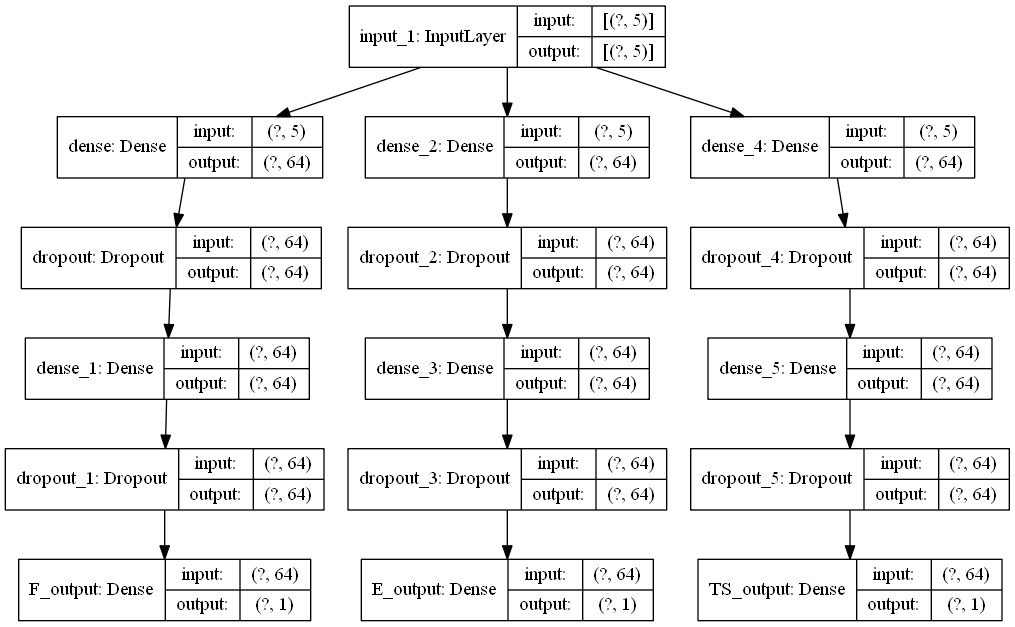
\includegraphics[height=8cm, keepaspectratio]{arch_1}
	\caption{Preliminary architecture for the NN} \label{fig:arch1}
\end{figure}


%______________________________________________________________________________________________
% Nomenclature introduced in this chapter:
\nomenclature[A]{ML}{Machine Learning}% 
\nomenclature[A]{SVM}{Support Vector Machines}%
\nomenclature[A]{NN}{Neural Network}%
\nomenclature[A]{MSE}{Mean Square Error}%
\nomenclature[A]{MAE}{Mean Absolute Error}%
\nomenclature[A]{SHAP}{Shapley Additive Explanations}%
\nomenclature[A]{ANOVA}{Analysis of Variance}%
\nomenclature[A]{IQR}{Interquartile Range}%

% Symbols introduced in this chapter:
\nomenclature[S]{$\phi_{j}$}{Shapley Value}
\nomenclature[S]{$\sigma_{T}$}{Maximum Tensile Stress}
\end{document}